\documentclass{beamer}
\usetheme{Warsaw}

\usepackage[utf8]{inputenc}
\usepackage{fancybox}
\usepackage{multimedia} 
\usepackage{subfig}
\usepackage{amsmath}

\usepackage[all]{xy}
\begin{document}


\title[Computergrafik] % (optional, only for long titles)
{Computergrafik

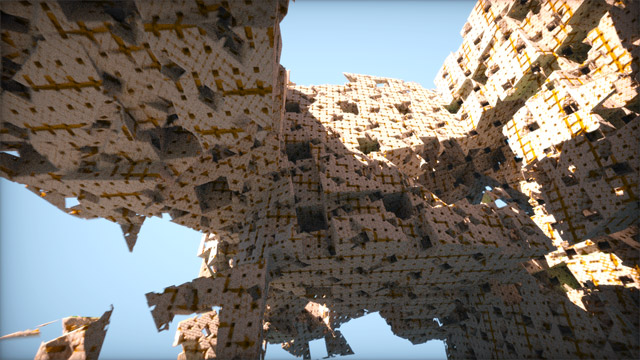
\includegraphics[scale=0.36]{images/cover}
}
\subtitle{}
\author[Dr. Johannes Riesterer] % (optional, for multiple authors)
{Dr.  rer. nat. Johannes Riesterer}

\date[KPT 2004] % (optional)
{}

\subject{Computergrafik}


\begin{frame}
    \frametitle{Computergrafik}
\framesubtitle{Echzeit Darstellung}
    \begin{block}{Echzeit Darstellung}
\begin{table}[h]
    \centering
    \begin{tabular}{|l|l|}
    \hline
    \textbf{Echtzeit-Typ} & \textbf{Eigenschaften} \\ \hline
    \textbf{Harte Echtzeit} & \begin{tabular}[c]{@{}l@{}}Zeitlimits zwingend, \\ Systemfehler bei Verpassen.\end{tabular} \\ \hline
    \textbf{Weiche Echtzeit} & \begin{tabular}[c]{@{}l@{}}Kleine Abweichungen erlaubt, \\ Leistung sinkt bei Überschreitung.\end{tabular} \\ \hline
    \end{tabular}
   % \caption{Definitionen von Echtzeitsystemen}
    \end{table}
    
\end{block}

\end{frame}


\begin{frame}
    \frametitle{Computergrafik}
\framesubtitle{Echzeit Darstellung}
    \begin{block}{Echzeit Darstellung}
Standard: $60$ Frames pro Sekunde bei einer Bildschirmauflösung von $4K=3840 \times 2160$ Pixel.  
D.h. $497.664.000$ Farbwerte müssen pro Sekunde berechnet und an das Ausgabegerät
geschickt werden. 
Kombination von Soft- und Hardware nötig.
\end{block}
\begin{table}[h]
    \centering
    \tiny % Schriftgröße ändern
    \begin{tabular}{|l|l|l|}
    \hline
    \textbf{GPU-Klasse} & \textbf{FP32-Leistung} & \textbf{FP64-Leistung} \\ \hline
    \textbf{Einsteiger- / Mittelklasse} & 2 - 10 TFLOPS & 0,1 - 1 TFLOPS \\ \hline
    \textbf{High-End-Gaming} & 10 - 20 TFLOPS & 1 - 5 TFLOPS \\ \hline
    \textbf{Workstation- / AI-GPUs} & 20 - 100 TFLOPS & 5 - 20 TFLOPS \\ \hline
    \textbf{Spezialisierte Hochleistung} & Mehrere 100 TFLOPS & Mehrere 20+ TFLOPS \\ \hline
    \end{tabular}
    \end{table}

\end{frame}




\begin{frame}{Aufbau und Funktionsweise einer GPU}
    \begin{itemize}
      \item \textbf{Architektur:} Viele einfache Rechenkerne in \textit{Streaming Multiprocessors (SM)}, optimiert für parallele Berechnung.
      \item \textbf{Speicherhierarchie:}
      \begin{itemize}
        \item \textit{Global Memory (VRAM)}: Großer, langsamer Speicher für die gesamte GPU.
        \item \textit{Shared Memory}: Schneller Zwischenspeicher pro SM.
        \item \textit{Register}: Klein, extrem schnell, lokal pro Kern.
      \end{itemize}
      \item \textbf{SIMD-Prinzip:} Gleiche Operation auf mehrere Daten gleichzeitig (Single Instruction, Multiple Data).
      \item \textbf{Thread-Modell:} Threads in \textit{Thread-Blocks} organisiert, diese in einem \textit{Grid}.
      \item \textbf{Spezialisierte Hardware:} Rasterisierung, Texturierung und Shading für Grafikoperationen.
    \end{itemize}
  \end{frame}



\begin{frame}
    \frametitle{Computergrafik}
\framesubtitle{}

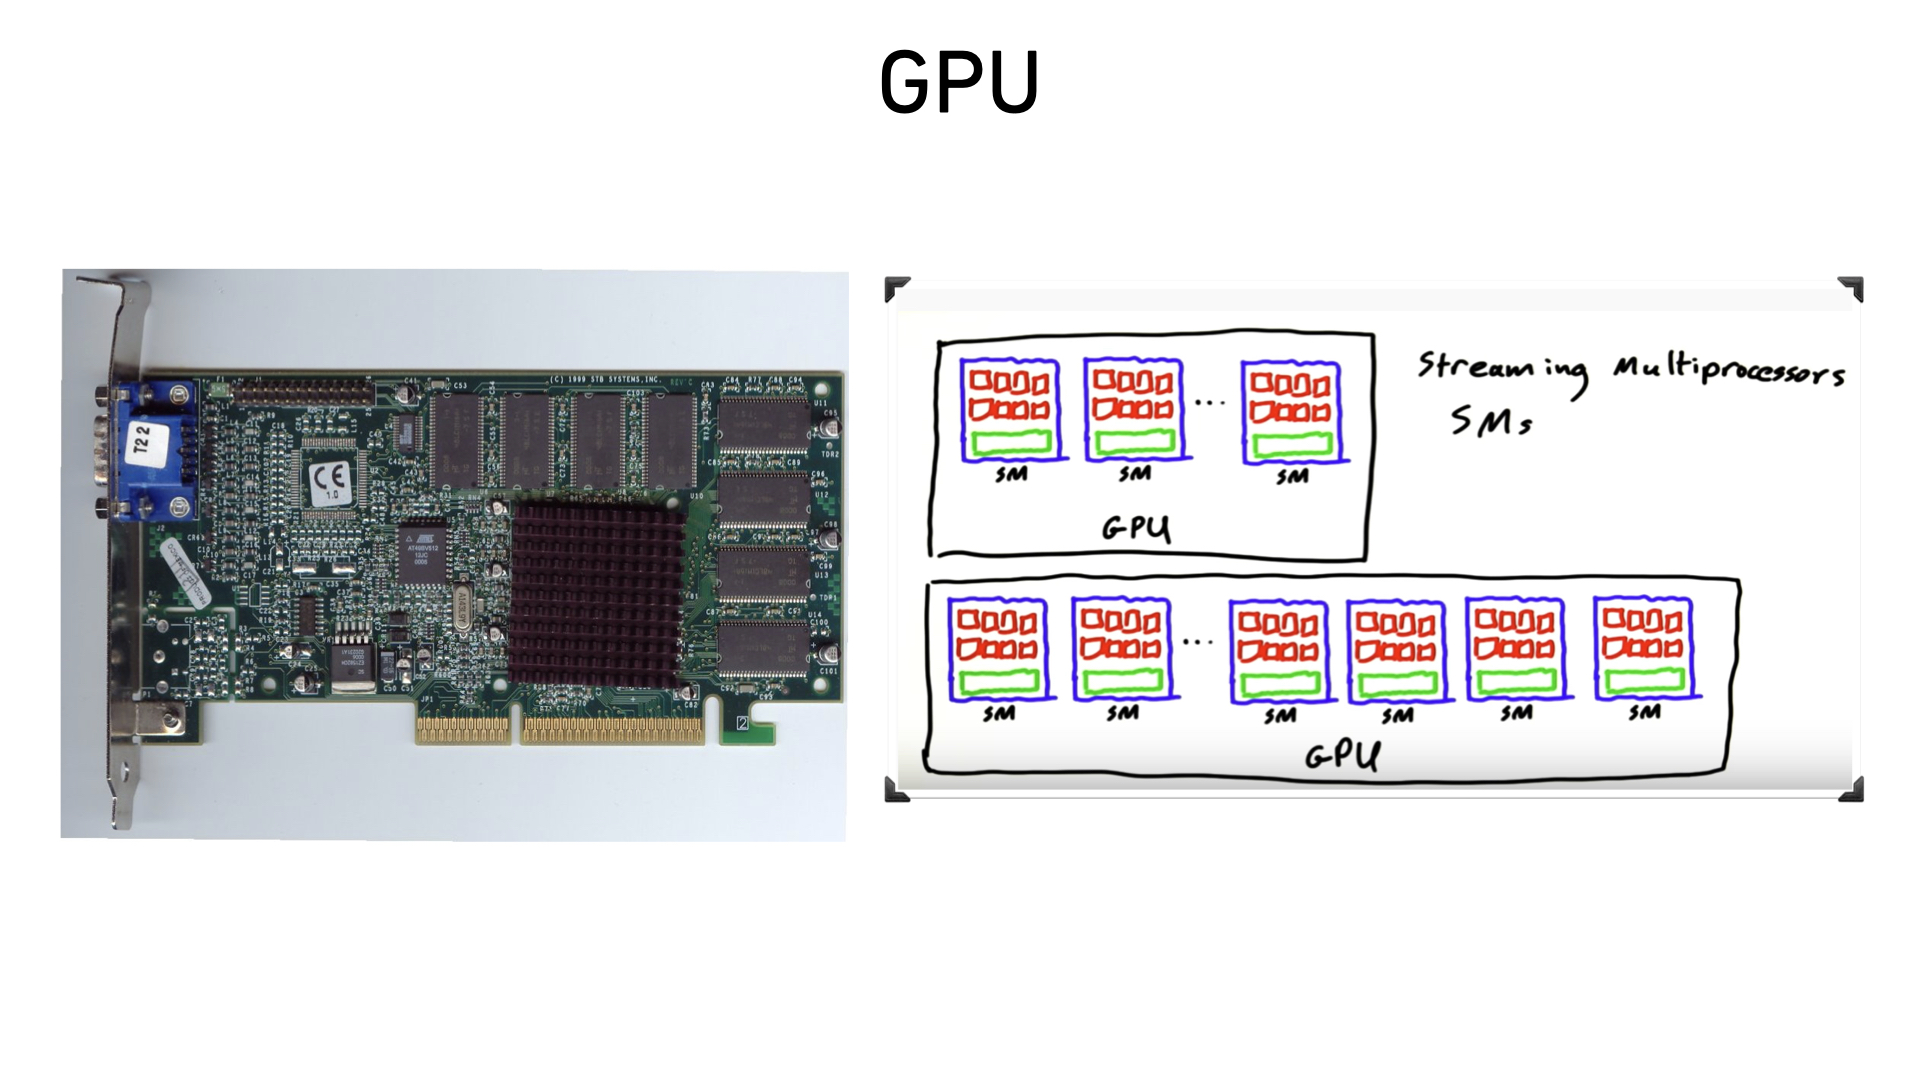
\includegraphics[scale=0.16]{images/Shaderday_Intro/Shaderday_Intro_004} \\
\end{frame}

\begin{frame}
    \frametitle{Computergrafik}
\framesubtitle{}

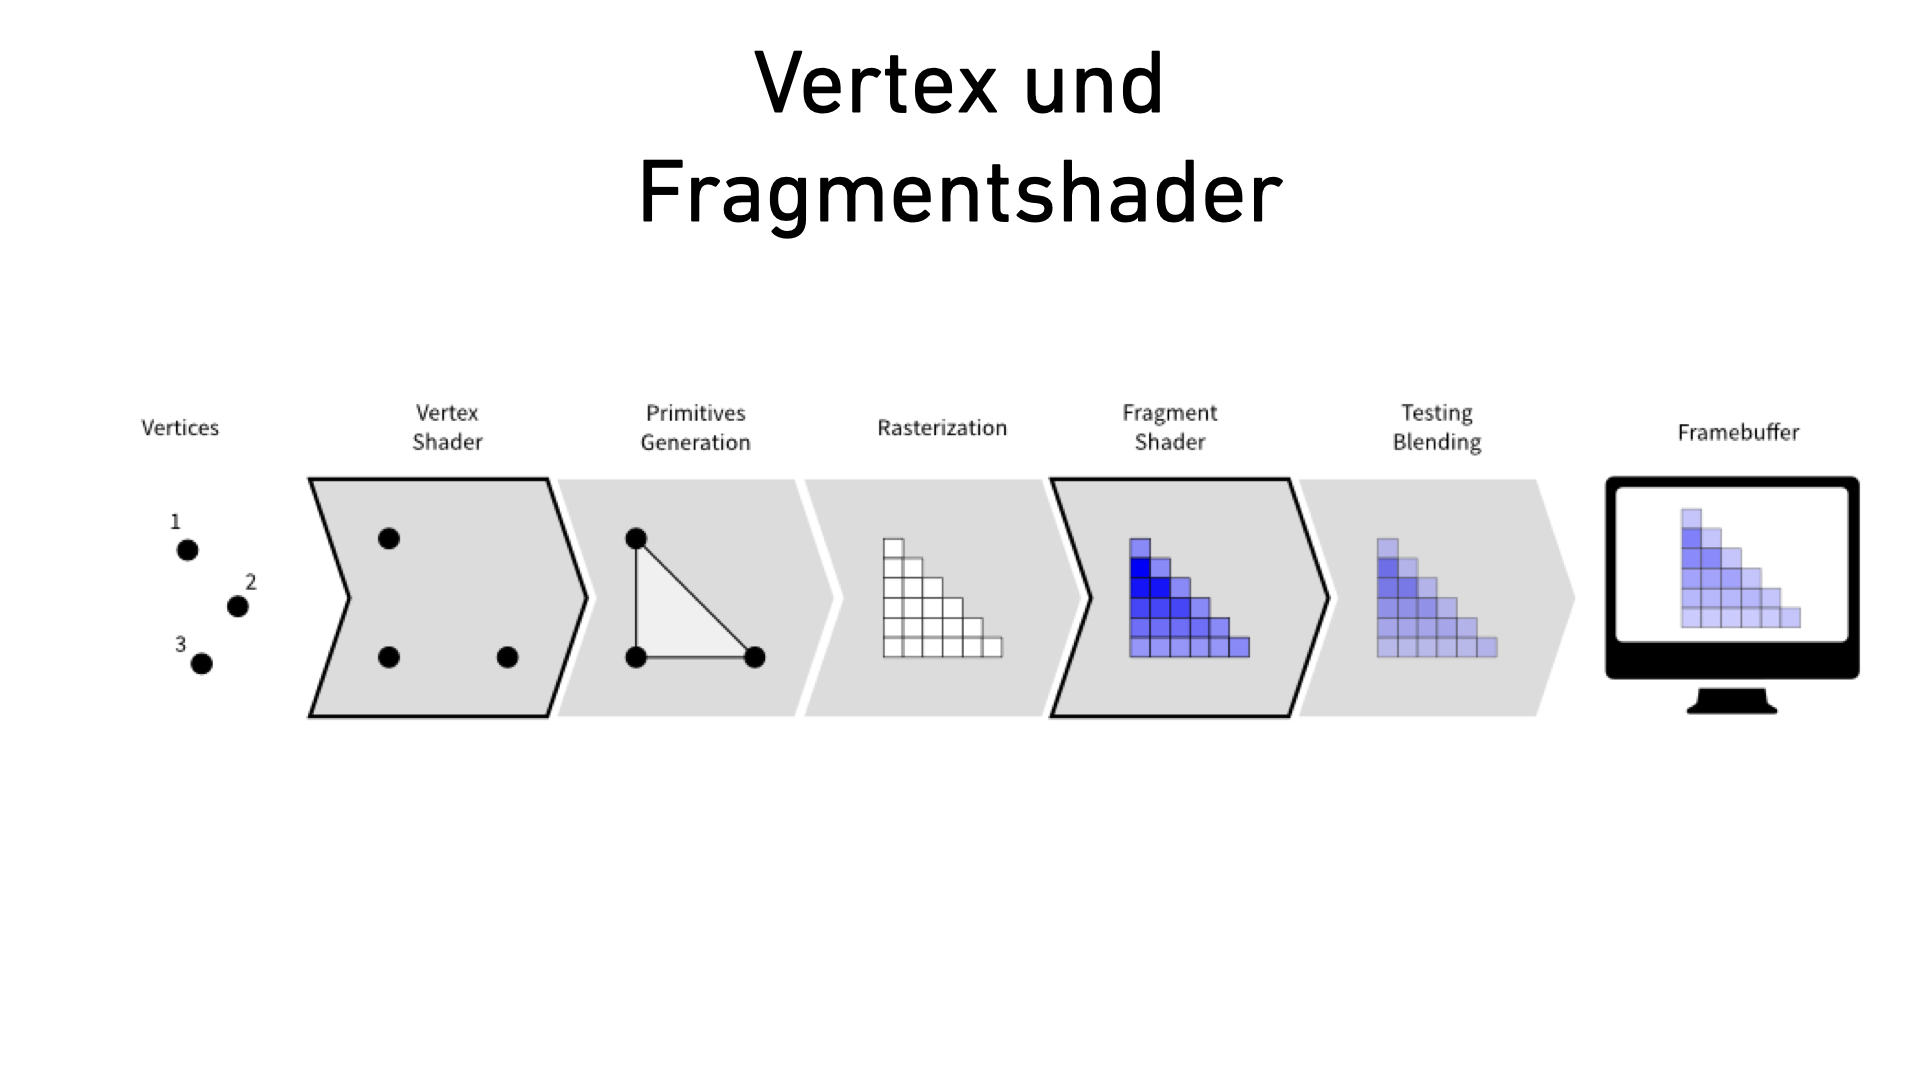
\includegraphics[scale=0.15]{images/Shaderday_Intro/Shaderday_Intro_007}

\end{frame}


\begin{frame}
    \frametitle{Computergrafik}
\framesubtitle{}

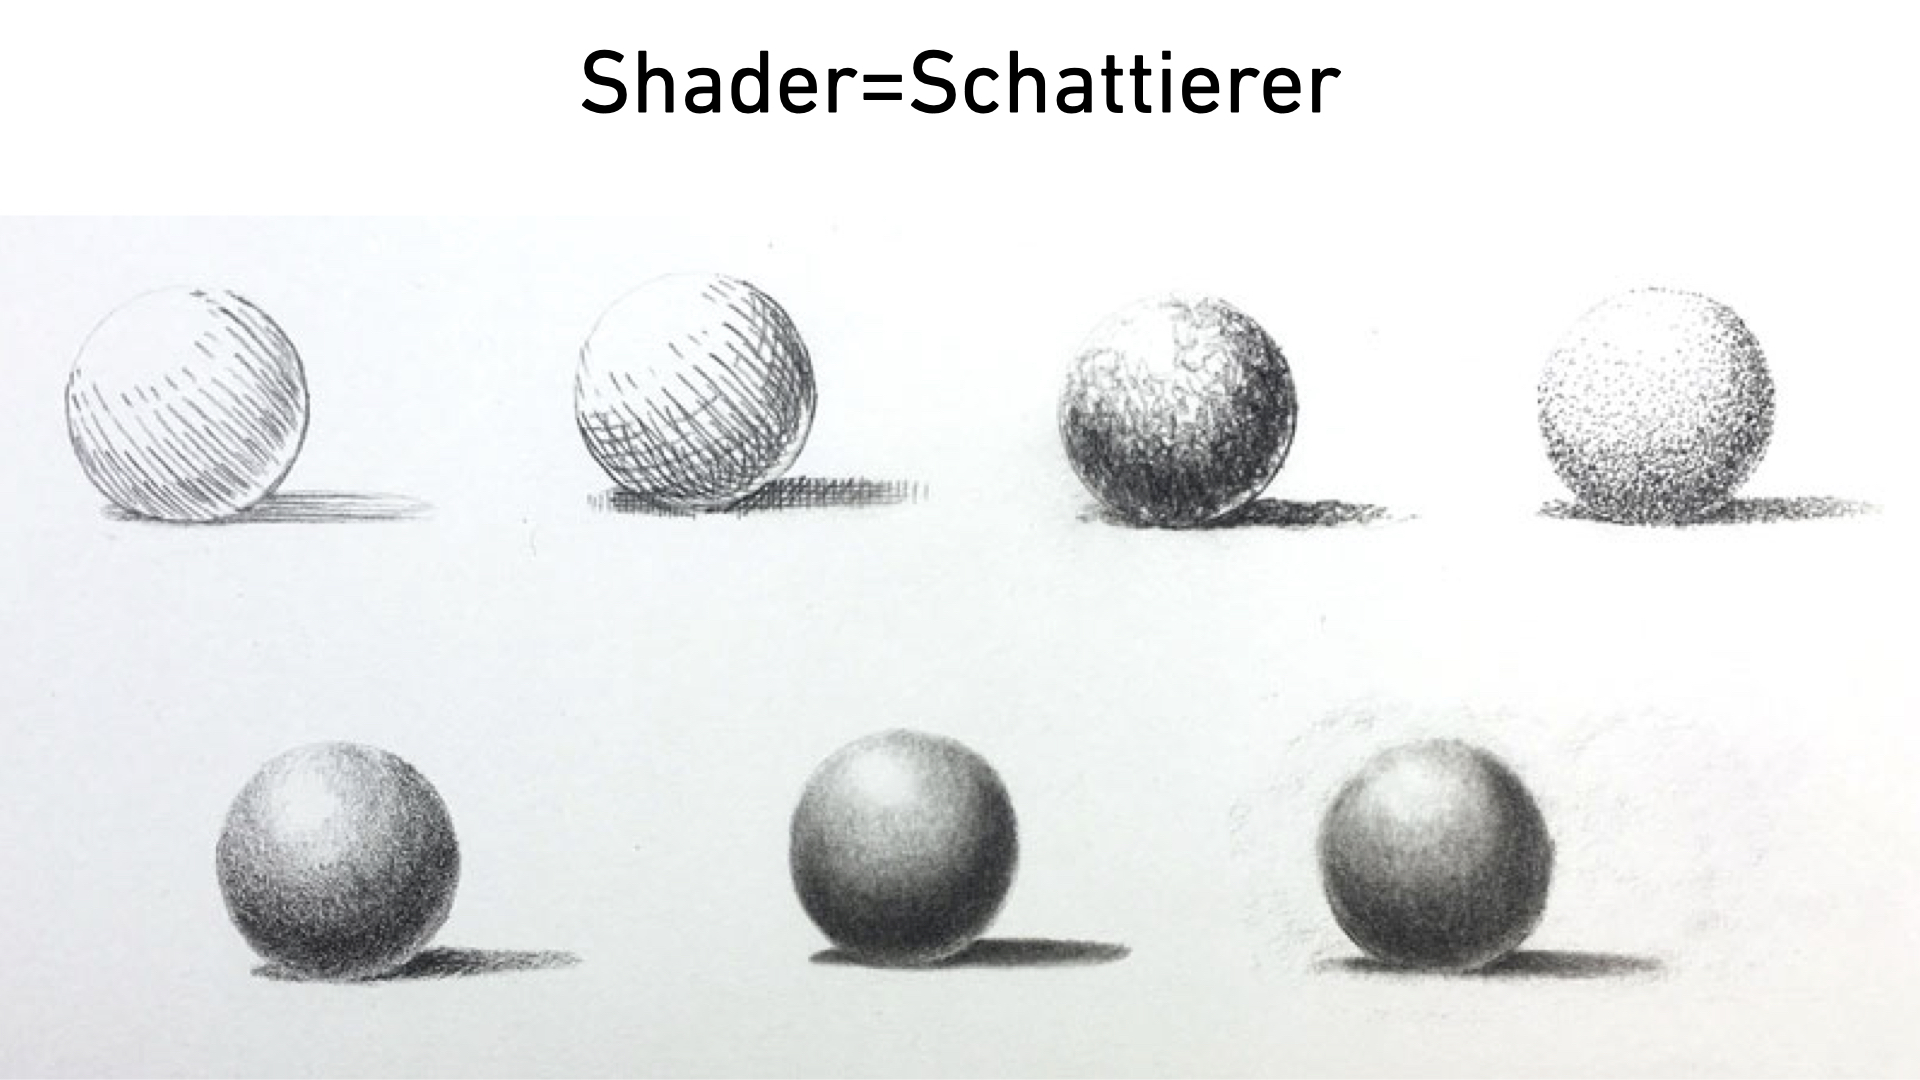
\includegraphics[scale=0.15]{images/Shaderday_Intro/Shaderday_Intro_001} 
\end{frame}



  
\begin{frame}
    \frametitle{ Shaderprogramm}
\framesubtitle{}
\begin{center}
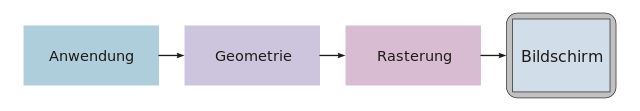
\includegraphics[scale=0.26]{images/cgpipeline_grob}
\\
\includegraphics[scale=0.20]{images/Zeichnung_Shaderpipeline}

\end{center}
\end{frame}

\begin{frame}
    \frametitle{OpenGL Pipeline}
\framesubtitle{}
    \begin{block}{}
\begin{center}
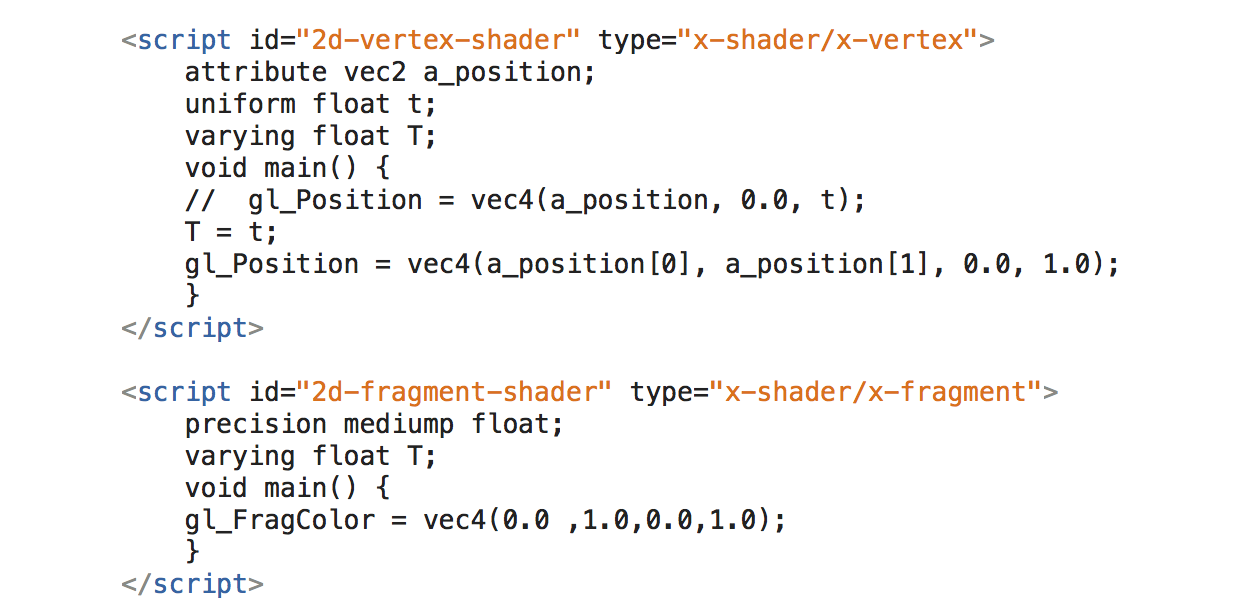
\includegraphics[scale=0.56]{images/shader}
\end{center}
\end{block}
\end{frame}


\begin{frame}
    \frametitle{HTML-Grundstruktur}
    \begin{block}{Beispielprogramm minimal\_fragmentshader.html}
        Beispielrogramm zur Darstellung eines grünen Dreiecks in WebGL.
        Vergleiche dazu das Programm  minimal\_fragmentshader.html
    \end{block}
    
    \begin{itemize}
        \item Der Code beginnt mit einer einfachen HTML-Struktur.
        \item Das \texttt{<canvas>} Element wird verwendet, um den Zeichenbereich für WebGL zu definieren.
        \item Zwei \texttt{<script>} Tags enthalten den Vertex- und Fragment-Shader, die die Zeichenoperationen steuern.
    \end{itemize}
\end{frame}

\begin{frame}[fragile]
    \frametitle{Vertex Shader}
    \begin{itemize}
        \item Der Vertex-Shader bestimmt die Position der Eckpunkte auf der Leinwand.
        \item \texttt{gl\_Position} legt die Position jedes Vertex im Raum fest.
    \end{itemize}
    \begin{verbatim}
    <script id="2d-vertex-shader" type="x-shader/x-vertex">
        attribute vec2 a_position;
        void main() {
            gl_Position = vec4(a_position.x, a_position.y, 0.0, 1.0);
        }
    </script>
    \end{verbatim}
\end{frame}

\begin{frame}[fragile]
    \frametitle{Fragment Shader}
    \begin{itemize}
        \item Der Fragment-Shader legt die Farbe der Pixel fest, die die Dreiecke füllen.
        \item In diesem Fall wird die Farbe auf Grün gesetzt: \texttt{vec4(0.0, 1.0, 0.0, 1.0)}.
    \end{itemize}
    \begin{verbatim}
    <script id="2d-fragment-shader" type="x-shader/x-fragment">
        precision mediump float;
        void main() {
            gl_FragColor = vec4(0.0, 1.0, 0.0, 1.0);
        }
    </script>
    \end{verbatim}
\end{frame}

\begin{frame}[fragile]
    \frametitle{WebGL Initialisierung und Shader-Kompilierung}
    \begin{itemize}
        \item Nach dem Laden des Dokuments wird der WebGL-Kontext erstellt.
        \item Die Shader werden kompiliert und das Programm wird verknüpft.
    \end{itemize}
    \begin{verbatim}
    gl = canvas.getContext("webgl");
    shaderScript = document.getElementById("2d-vertex-shader");
    vertexShader = gl.createShader(gl.VERTEX_SHADER);
    gl.shaderSource(vertexShader, shaderScript.text);
    gl.compileShader(vertexShader);
    \end{verbatim}
\end{frame}

\begin{frame}[fragile]
    \frametitle{Erstellen und Binden des Buffers}
    \begin{itemize}
        \item Ein Buffer wird erstellt, um die Vertex-Daten zu speichern.
        \item Die Positionen der Eckpunkte des Dreiecks werden in den Buffer geladen.
    \end{itemize}
    \begin{verbatim}
    gl.bindBuffer(gl.ARRAY_BUFFER, buffer);
    gl.bufferData(gl.ARRAY_BUFFER, 
        new Float32Array([
            -1.0, -1.0,
            1.0, -1.0,
            -1.0, 1.0,
            -1.0, 1.0,
            1.0, -1.0,
            1.0, 1.0]), 
        gl.STATIC_DRAW);
    \end{verbatim}
\end{frame}

\begin{frame}
    \frametitle{Zeichnen des Dreiecks}
    \begin{itemize}
        \item Die Vertex-Attribute werden aktiviert und an den Shader übergeben.
        \item Schließlich wird das Dreieck mit \texttt{gl.drawArrays()} gezeichnet.
    \end{itemize}
\end{frame}



\begin{frame}{Echzeit Darstellung}
    \begin{block}{Animation}
    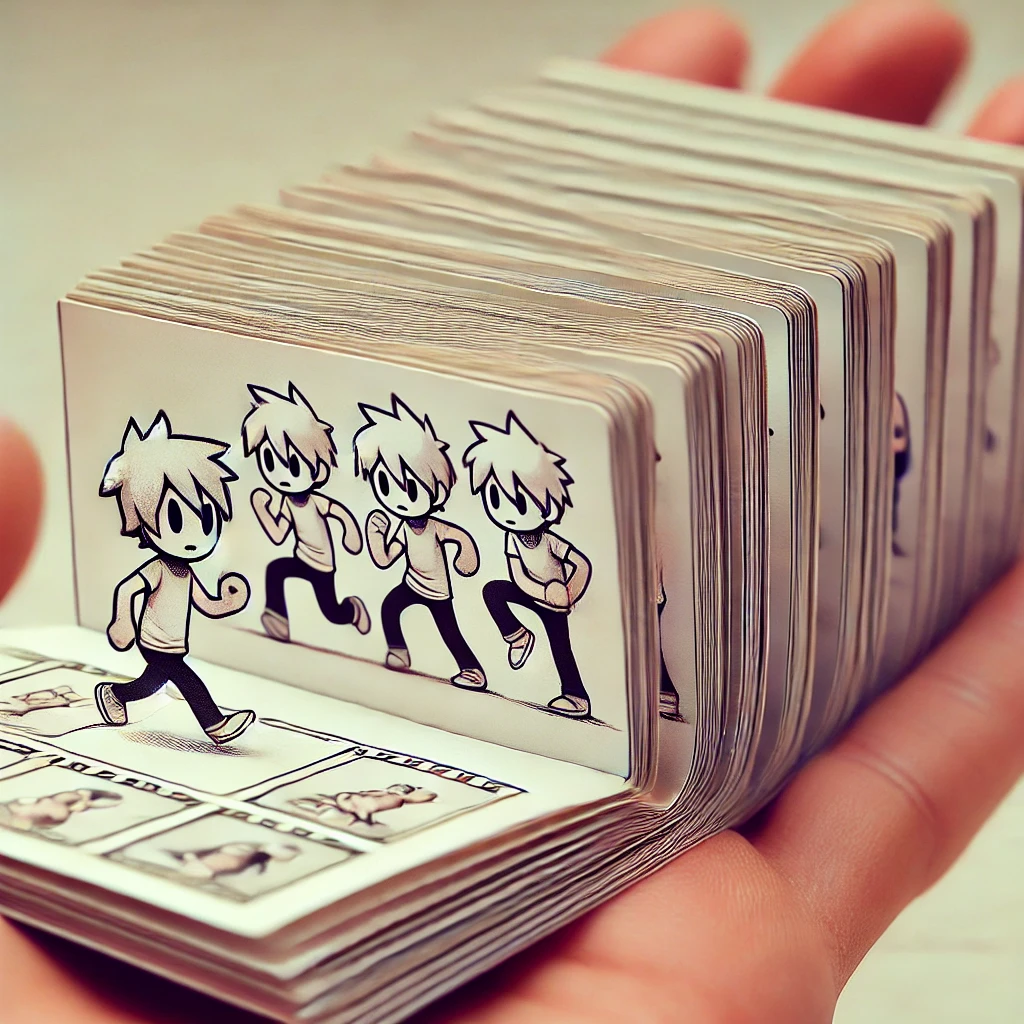
\includegraphics[scale=0.2]{images/animation.png} 
\end{block}

\end{frame}


  \begin{frame}{Echzeit Darstellung}
    \begin{block}{Animation}
   Bewegungsabläufe werden durch eine Abfolge von statischen Bildern erzeugt, die so schnell nacheinander angezeigt werden, dass im Gehirn der Eindruck einer kontinuierlichen Bewegung entsteht. 
    Diese Abfolge von Bildern wird als Frames bezeichnet. 
    Die Illusion einer flüssigen Bewegung wird durch ein Phänomen in unserem visuellen System erzeugt, das als "Bewegungs-Nachbilder" oder auch "Persistence of Vision" bekannt ist.
\end{block}
\end{frame}
  

\begin{frame}{Begriff der Animation}
    \begin{itemize}
      \item \textbf{Illusion im Gehirn:}
      \begin{itemize}
        \item \textbf{Nachbilder im Auge:} Bilder verbleiben kurzzeitig auf der Netzhaut (ca. 1/25 Sekunde).
        \item \textbf{Verarbeitung im Gehirn:} 
        \begin{itemize}
          \item Aufeinanderfolgende Bilder werden kombiniert.
          \item Übergänge werden als kontinuierliche Bewegung interpretiert.
        \end{itemize} 
        \item \textbf{Bewegungswahrnehmung:} Spezialisierte Neuronen erkennen Bildunterschiede als Bewegung.
      \end{itemize}
      \item \textbf{Bildrate (Frames per Second, FPS):}
      \begin{itemize}
        \item \textbf{Unter 12 FPS:} Einzelbilder werden als ruckartig wahrgenommen.
        \item \textbf{Ab 24 FPS:} Flüssige Bewegung, typisch für Filme.
        \item \textbf{60 FPS:} Realistische Darstellung, z.B. in Computerspielen.
      \end{itemize}
    \end{itemize}
  \end{frame}
  

  \begin{frame}
    \frametitle{Echtzeit}
\framesubtitle{}
    \begin{block}{Chronofotografie}
        Die Chronofotografie (auch Fotochronografie) bezeichnet die fotografische Dokumentation von Bewegungen oder Prozessen, heute hauptsächlich als Hochgeschwindigkeitsfotografie. 
\end{block}

\begin{block}{Chronofotografie}
    In der Entwicklung der Fotografie wurden in den 1870er und 1880er Jahren durch empfindliche Photomaterialien und schnelle Kameraverschlüsse sogenannte Augenblicks- oder Momentfotografien möglich, Aufnahmen bewegter Objekte.
\end{block}
\end{frame}


\begin{frame}
    \frametitle{Computergrafik}
\framesubtitle{}
    \begin{block}{Chronofotografie}
        Muybridge gelang 1878 der Nachweis, dass ein Pferd im Galopp kurzzeitig mit allen vier Hufen vom Boden abhebt. Diese frühen Serienaufnahmen lieferten wichtige Impulse für die Entwicklung der bewegten Bilder und waren damit auch Vorläufer des Kinofilms. 
    \end{block}
    \begin{center}
        
        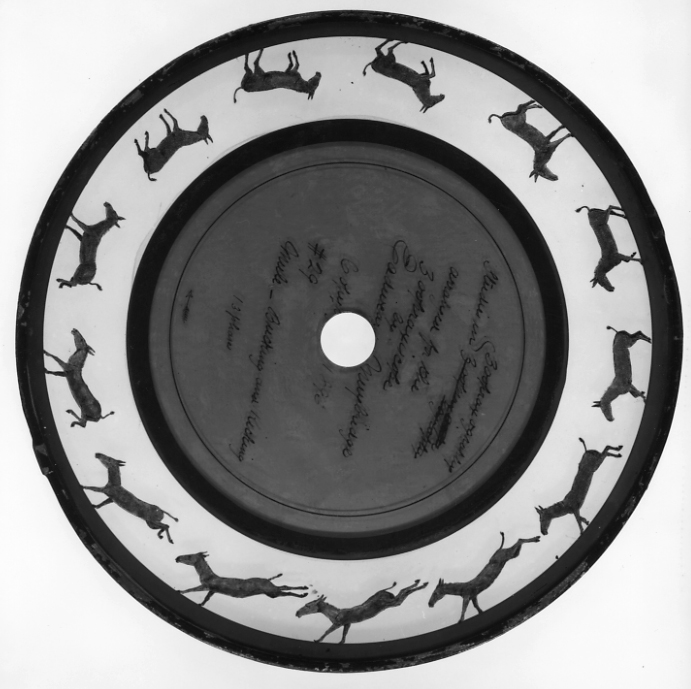
\includegraphics[scale=0.36]{images/Zoopraxiscope.jpg}
    \end{center}
   
\end{frame}


\begin{frame}{Echzeit Darstellung}
    \begin{block}{Sprite Animation}
    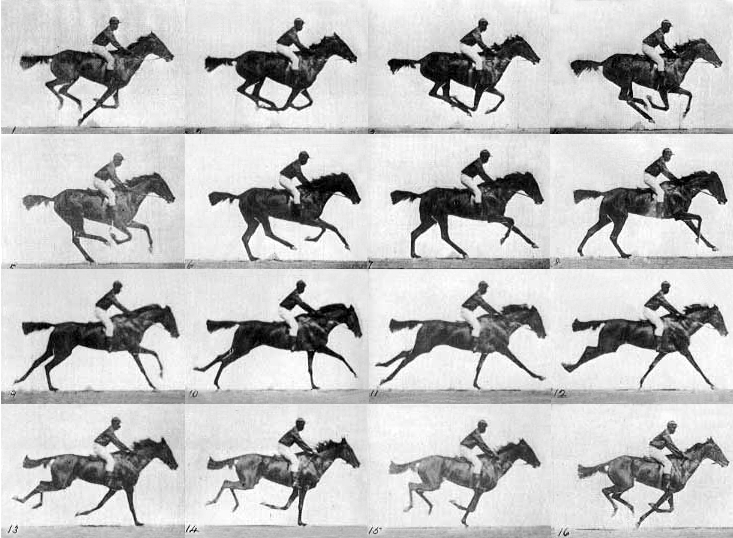
\includegraphics[scale=0.4]{images/horse} 
\end{block}

\end{frame}


\begin{frame}
    \frametitle{Was ist Sprite Animation?}
    \begin{itemize}
        \item Sprite-Animation ist eine Technik, bei der Bilder (Sprites) in einer Sequenz angezeigt werden, um Bewegung darzustellen.
        \item Ein Sprite-Sheet ist ein Bild, das mehrere Sprites in einem Raster enthält.
        \item Jedes Sprite repräsentiert eine einzelne Bildsequenz (Frame) der Animation.
        \item Die Bilder werden schnell hintereinander gezeigt, um die Illusion von Bewegung zu erzeugen.
    \end{itemize}
\end{frame}

\begin{frame}
    \frametitle{Funktionsweise}
    \begin{itemize}
        \item Ein Sprite-Sheet wird in Reihen und Spalten unterteilt, wobei jeder Abschnitt einen Frame der Animation darstellt.
        \item Eine Schleife wechselt durch die Frames des Sprite-Sheets basierend auf einer Bildrate (fps).
        \item Die Position und Skalierung des Sprites können ebenfalls animiert werden.
    \end{itemize}
\end{frame}

\begin{frame}
    \frametitle{Vorteile der Sprite Animation}
    \begin{itemize}
        \item Spart Speicherplatz, da mehrere Animationen in einem Bild gespeichert werden können.
        \item Effizient für Spiele und Anwendungen, die viele kleine Animationssequenzen benötigen.
        \item Unterstützt einfache Bewegungsanimationen ohne aufwendige Rechenleistung.
    \end{itemize}
\end{frame}


\begin{frame}
    \frametitle{HTML-Grundstruktur}
    \begin{block}{Beispielprogramm SpriteAnimator}
        Vergleiche dazu das Programm  SpriteAnimator
    \end{block}
    \begin{itemize}
        \item Das Skript verwendet die HTML5 \texttt{<canvas>} API, um eine Sprite-Animation auf einer Leinwand zu zeichnen.
        \item Der \texttt{<canvas>} wird über CSS mit einer Breite von 280px und einer Höhe von 133px gestylt.
        \item Ein \texttt{<img>} Tag lädt das Bild, das als Sprite-Sheet für die Animation verwendet wird.
    \end{itemize}
\end{frame}

\begin{frame}[fragile]
    \frametitle{CSS-Styling}
    \begin{itemize}
        \item Das Canvas-Element hat eine festgelegte Breite und Höhe sowie eine Randlinie.
    \end{itemize}
    \begin{verbatim}
    <style>
      #myCanvas {
        width: 280px;
        height: 133px;
        border: 2px solid #000000;
      }
    </style>
    \end{verbatim}
\end{frame}

\begin{frame}
    \frametitle{Die Animation-Klasse}
    \begin{itemize}
        \item Die \texttt{Animation}-Klasse wird erstellt, um die Animation zu handhaben.
        \item Sie nimmt mehrere Parameter entgegen: das Bild, die Bildrate (\texttt{fps}), die Breite und Höhe des Sprites, die Skalierung, die Anzahl der Zeilen und Spalten im Sprite-Sheet, sowie die Position des Sprites auf dem Canvas.
    \end{itemize}
\end{frame}

\begin{frame}[fragile]
    \frametitle{Update-Methode der Animation}
    \begin{itemize}
        \item Die \texttt{update}-Methode aktualisiert den aktuellen Sprite-Index basierend auf der verstrichenen Zeit.
        \item Sie berechnet, wann der nächste Frame basierend auf den \texttt{fps} angezeigt werden soll.
    \end{itemize}
    \begin{verbatim}
    Animation.prototype.update = function(dt) {
        this.elapsedTime += dt;
        if (1000.0 / this.fps - this.elapsedTime < 0.0) {
            this.index += 1;
            this.index = this.index % (this.nRows * this.nColls);
            this.elapsedTime = 0.0;
        }
    };
    \end{verbatim}
\end{frame}

\begin{frame}[fragile]
    \frametitle{Draw-Methode der Animation}
    \begin{itemize}
        \item Die \texttt{draw}-Methode zeichnet den aktuellen Frame der Animation.
        \item Sie berechnet die Position des aktuellen Frames auf dem Sprite-Sheet und zeichnet das entsprechende Bild auf das Canvas.
    \end{itemize}
    \begin{verbatim}
    Animation.prototype.draw = function(ctx) {
        var i = Math.floor(this.index / this.nColls);
        var j = this.index % this.nColls;
        ctx.drawImage(this.spriteSheet, 
                      j * this.width, 
                      i * this.height, 
                      this.width, 
                      this.height, 
                      this.posX, 
                      this.posY, 
                      this.scale * this.width, 
                      this.scale * this.height);
    };
    \end{verbatim}
\end{frame}

\begin{frame}
    \frametitle{Der gameLoop}
    \begin{itemize}
        \item Der \texttt{gameLoop} wird kontinuierlich ausgeführt, um die Animation zu aktualisieren und zu rendern.
        \item Der Loop nutzt \texttt{requestAnimationFrame}, um die Bildrate zu steuern und die Animation flüssig darzustellen.
        \item Jede Iteration aktualisiert die Animation und zeichnet den neuen Frame auf das Canvas.
    \end{itemize}
\end{frame}

\begin{frame}[fragile]
    \frametitle{Code des Game Loops}
    \begin{verbatim}
    function gameLoop() {
        window.requestAnimationFrame(gameLoop);
        ctx.clearRect(0, 0, canvas.width, canvas.height);
        
        d = new Date();
        var currentTime = d.getTime();
        var dt = currentTime - prevTime;
        anim.update(dt);
        anim.draw(ctx);
        prevTime = currentTime;
    }
    \end{verbatim}
\end{frame}


\end{document}
